%% ============================================================ 7 HYPOTHESIS TESTING
\clearpage
\inchap{Hypothesis Testing}
\section{Terminology}
\begin{center}\ba\small
\begin{tabular}{|M{3.8cm}|L{11.4cm}|}\hline
\textbf{Term} & \textbf{Meaning}\\\Xhline{2pt}
Null hypothesis $\Hz$ & the claim assumed true: $\Hz:\ \mu=\mu_{0}$\\\hline
Alternative hypothesis $\Ho$ & what we look for evidence of: $\mu<\mu_{0}$, $\mu>\mu_{0}$ (1-tail) or $\mu\neq\mu_{0}$ (2-tail)\\\hline
Test statistic & $\Xb$ (or $Z$), whose distribution is found assuming $\Hz$ is true\\\hline
Level of significance $\alpha$ & probability of rejecting $\Hz$ when $\Hz$ is true; given in the question\\\hline
Critical region & values of the test statistic for which $\Hz$ is rejected; boundary = critical value\\\hline
$p$-value & probability, assuming $\Hz$ true, of a test statistic at least as extreme as the one observed; smallest level at which $\Hz$ is rejected\\\hline
\end{tabular}\end{center}
\section{Formulating the Hypotheses}
\begin{center}\ba\small
\begin{tabular}{|L{6.4cm}|M{3.2cm}|M{3.4cm}|}\hline
\textbf{Wording} & $\Ho$ & \textbf{Type}\\\Xhline{2pt}
decreased, less than, lower, overstated & $\mu<\mu_{0}$ & 1-tail (lower)\\\hline
increased, more than, greater, understated & $\mu>\mu_{0}$ & 1-tail (upper)\\\hline
changed, different, not correct, biased & $\mu\neq\mu_{0}$ & 2-tail\\\hline
\end{tabular}\end{center}
\sidenote{Define $\mu$ in context (e.g.\ ``$\mu$ is the population mean mass''). $\Hz$ always uses ``$=$''.}\par
\section{Test Statistic and Its Distribution}
\begin{center}\bba\small
\begin{tabular}{|L{5.6cm}|M{5.2cm}|L{4.4cm}|}\hline
\textbf{Situation} & \textbf{Distribution under $\Hz$} & \textbf{Say}\\\Xhline{2pt}
Normal population, $\sigma^{2}$ known & $\Xb\sim\No{\mu_{0}}{\dfrac{\sigma^{2}}{n}}$ & any $n$\\\hline
Any population, $n$ large, $\sigma^{2}$ known & $\Xb\sim\No{\mu_{0}}{\dfrac{\sigma^{2}}{n}}$ approximately by CLT & ``by CLT''\\\hline
Any population, $n$ large, $\sigma^{2}$ unknown & $\Xb\sim\No{\mu_{0}}{\dfrac{s^{2}}{n}}$ approximately by CLT & ``by CLT''; $s^{2}$ unbiased estimate\\\hline
\end{tabular}\end{center}
\clearpage
\section{The Test: $p$-value and Critical Region}
\begin{center}\begin{tikzpicture}
\begin{groupplot}[group style={group size=3 by 1,horizontal sep=0.9cm},nc,width=5.5cm,height=2.9cm]
\nextgroupplot[title={$\Ho:\mu<\mu_{0}$},title style={font=\small}]
\addplot[fill=red!30,draw=none,domain=-3.4:-1.645]{\nf{0}}\closedcycle;
\addplot[black,semithick]{\nf{0}};
\node[below] at (axis cs:0,0){$\mu_{0}$};\node[below,font=\scriptsize] at (axis cs:-1.645,0){$c$};
\node[font=\scriptsize,red!60!black] at (axis cs:-2.4,0.2){$\alpha$};
\nextgroupplot[title={$\Ho:\mu>\mu_{0}$},title style={font=\small}]
\addplot[fill=red!30,draw=none,domain=1.645:3.4]{\nf{0}}\closedcycle;
\addplot[black,semithick]{\nf{0}};
\node[below] at (axis cs:0,0){$\mu_{0}$};\node[below,font=\scriptsize] at (axis cs:1.645,0){$c$};
\node[font=\scriptsize,red!60!black] at (axis cs:2.4,0.2){$\alpha$};
\nextgroupplot[title={$\Ho:\mu\neq\mu_{0}$},title style={font=\small}]
\addplot[fill=red!30,draw=none,domain=-3.4:-1.96]{\nf{0}}\closedcycle;
\addplot[fill=red!30,draw=none,domain=1.96:3.4]{\nf{0}}\closedcycle;
\addplot[black,semithick]{\nf{0}};
\node[below] at (axis cs:0,0){$\mu_{0}$};\node[below,font=\scriptsize] at (axis cs:-1.96,0){$c_{1}$};\node[below,font=\scriptsize] at (axis cs:1.96,0){$c_{2}$};
\node[font=\scriptsize,red!60!black] at (axis cs:-2.7,0.2){$\tfrac\alpha2$};\node[font=\scriptsize,red!60!black] at (axis cs:2.7,0.2){$\tfrac\alpha2$};
\end{groupplot}\end{tikzpicture}\end{center}
\begin{center}\ba\small
\begin{tabular}{|M{3.2cm}|M{4.2cm}|M{3.6cm}|M{3.8cm}|}\hline
 & \textbf{Lower tail} & \textbf{Upper tail} & \textbf{2-tail}\\\Xhline{2pt}
$p$-value & $\Pp{\Xb\leqslant\xb}$ & $\Pp{\Xb\geqslant\xb}$ & $2\Pp{\Xb\leqslant\xb}$ if $\xb<\mu_{0}$;\ $2\Pp{\Xb\geqslant\xb}$ if $\xb>\mu_{0}$\\\hline
Reject $\Hz$ if & \multicolumn{3}{c|}{$p$-value $\leqslant\alpha$}\\\hline
Critical region & $\Xb\leqslant c$,\ $\Pp{\Xb\leqslant c}=\alpha$ & $\Xb\geqslant c$,\ $\Pp{\Xb\geqslant c}=\alpha$ & $\Xb\leqslant c_{1}$ or $\Xb\geqslant c_{2}$; each tail $\tfrac\alpha2$\\\hline
Reject $\Hz$ if & \multicolumn{3}{c|}{$\xb$ lies in the critical region}\\\hline
\end{tabular}\end{center}
\begin{theorem}[before skip=3mm,after skip=3mm]{$p$-value of a two-tailed test}
\[\text{$p$-value (two-tailed test)}=2\times\text{$p$-value (one-tailed test)}\]
\end{theorem}
\begin{theorem}[before skip=3mm,after skip=3mm]{Steps of a test}
\begin{tabular}{@{}l@{\ \ }l@{}}
1 & $\Hz:\ \mu=\mu_{0}$,\ \ $\Ho:\ \mu\ \square\ \mu_{0}$;\ define $\mu$;\ state $\alpha$\\
2 & distribution of $\Xb$ under $\Hz$ (with reason: normal population / CLT)\\
3 & $p$-value from the GC \ (or critical region)\\
4 & compare: $p\leqslant\alpha\Rightarrow$ reject $\Hz$; \ $p>\alpha\Rightarrow$ do not reject $\Hz$\\
5 & conclusion \textbf{in context}\\
\end{tabular}
\end{theorem}
\begin{center}\ba\small
\begin{tabular}{|L{3.6cm}|L{11.6cm}|}\hline
\textbf{Result} & \textbf{Conclusion (in context)}\\\Xhline{2pt}
Reject $\Hz$ & there is sufficient evidence, at the $\alpha$ level of significance, to conclude that [$\Ho$ in words]\\\hline
Do not reject $\Hz$ & there is insufficient evidence, at the $\alpha$ level of significance, to conclude that [$\Ho$ in words]\\\hline
\end{tabular}\end{center}
\sidenote{Never write ``accept $\Hz$'' or ``$\Hz$ is true / proven''.}\par
\gcs{\gckey{STAT} $\to$ \gc{TESTS} $\to$ \gc{1:Z-Test}.\ \gc{Inpt:Stats}; enter \gc{$\mu$0}, \gc{$\sigma$} (use $s$ if $\sigma$ unknown, large $n$), \gc{$\bar{x}$}, \gc{n}; choose \gc{$\neq\mu$0}, \gc{$<\mu$0} or \gc{$>\mu$0} to match $\Ho$; \gc{Calculate} gives $z$ and $p$. With raw data use \gc{Inpt:Data} with the list; for a frequency table first run \gc{1-Var Stats L1,L2} to get $\bar{x}$ and \gc{Sx}, then use \gc{Inpt:Stats}.}
\clearpage
\noindent\exlab \hfill{\small[N2016/H1/10]}\par
\noindent A scientist claims that the mean top speed of cheetahs, in km/h, is 95. The top speed of each cheetah in a random sample of 40 cheetahs is recorded and the mean is found to be 96.3. It is known that the top speeds of cheetahs are normally distributed with standard deviation 4.1.\par
\noindent(i) Test the scientist's claim at the 5\% significance level.\hfill[4]
\par\smallskip
\begin{flushleft}
Let $X$ denote the top speed of a randomly selected cheetah in km/h, with population mean $\mu$ km/h.\par\smallskip
$\Hz:\ \mu=95$\\
$\Ho:\ \mu\neq95$\par\smallskip
Conduct a 2-tailed test at the 5\% level of significance.\par\smallskip
Test statistic:\\
Under $\Hz$, \textcolor{gray}{\textit{(since $n=40$ is large, by central limit theorem,)}}\\[4pt]
$\Xb\sim\No{95}{\dfrac{4.1^{2}}{40}}$ \textcolor{gray}{\textit{approximately}}\par\smallskip
\begin{center}\begin{tikzpicture}[x=1.1cm,y=4.4cm]
\fill[red!45] (1.96,0) -- plot[domain=1.96:3.4,samples=40] (\x,{exp(-\x*\x/2)/sqrt(2*pi)}) -- (3.4,0) -- cycle;
\fill[red!45] (-3.4,0) -- plot[domain=-3.4:-1.96,samples=40] (\x,{exp(-\x*\x/2)/sqrt(2*pi)}) -- (-1.96,0) -- cycle;
\fill[blue!50] (2.3,0) -- plot[domain=2.3:3.4,samples=40] (\x,{exp(-\x*\x/2)/sqrt(2*pi)}) -- (3.4,0) -- cycle;
\draw[->] (-3.6,0) -- (3.9,0) node[right]{$\bar{x}$};
\draw[thick] plot[domain=-3.4:3.4,samples=100] (\x,{exp(-\x*\x/2)/sqrt(2*pi)});
\draw[dashed] (0,0) -- (0,{1/sqrt(2*pi)});
\node[below] at (0,0){$95$};
\node[below] at (-1.96,0){$c_{1}$}; \node[below] at (1.85,0){$c_{2}$};
\draw (2.3,0) -- (2.3,-0.03); \node[below] at (2.45,-0.02){$96.3$};
\draw (-2.3,0.015) -- (-2.9,0.17) node[above,red!60!black]{$\dfrac{\alpha}{2}=0.025$};
\draw (2.1,0.03) -- (2.2,0.2) node[above,red!60!black]{$\dfrac{\alpha}{2}=0.025$};
\draw (2.7,0.007) -- (3.4,0.06) node[above,blue!60!black]{$\dfrac{p\text{-value}}{2}$};
\end{tikzpicture}\end{center}
Reject $\Hz$ if $p$-value $\leqslant$ 5\% level of significance.\par\smallskip
By GC, $p$-value $=0.0449$\par\smallskip
Thus, since $p$-value $<5\%$, we reject $\Hz$ at the 5\% level of significance. There is sufficient evidence to conclude that the mean top speed of cheetahs is not 95km/h. So the scientist's claim is not valid.
\end{flushleft}
\noindent\begin{minipage}{\textwidth}
{\large\bfseries\color{blue!50!black}Common Definitions}\par\smallskip
\centering\renewcommand{\arraystretch}{1.05}\footnotesize
\begin{tabular}{|L{2.3cm}|L{6.45cm}|L{6.45cm}|}\hline
\textbf{Term} & \textbf{Template} & \textbf{Definition (in context)}\\\Xhline{2pt}
Random sample & every member of the population is equally likely to be chosen and the selections are independent. & each cheetah is equally likely to be chosen and the selections are independent\\\hline
Level of significance & there is a probability of $\alpha\%$ that we wrongly reject $\Hz$, when $\Hz$ is in fact true. & there is a probability of 5\% that we wrongly conclude that the population mean top speed of cheetahs is not 95km/h when it is actually 95km/h.\\\hline
$p$-value & it is the probability that the test statistic is as extreme or more extreme than the observed value given that $\Hz$ is true.\newline \textbf{OR}\newline It is the smallest level of significance such that $\Hz$ is rejected. & it is 2 times the probability that the sample mean top speed of cheetahs is at least 96.3km/h when the population mean top speed is 95km/h.\newline \textbf{OR}\newline It is the smallest level of significance to conclude that the mean top speed of cheetahs is not 95km/h.\\\hline
Unbiased estimate & it is an estimate whose expected value is equal to the population parameter it is estimating. & \\\hline
\end{tabular}
\end{minipage}
\begin{landscape}
\section{Reverse Questions}
\noindent Reverse questions in hypothesis testing ask us to find the range of some variable, given that $\Hz$ is rejected or $\Hz$ is not rejected. Each question below uses the data of Example 7.1 [N2016/H1/10] with one quantity replaced by an unknown. In every case $\Hz:\mu=\mu_{0}$, $\Ho:\mu\neq\mu_{0}$ (2-tailed), and ``the scientist's claim is not valid'' means $\Hz$ is rejected.\par\smallskip
{\renewcommand{\arraystretch}{1.15}\scriptsize
\setlength{\jot}{1pt}
\begin{longtable}{|M{1.0cm}|L{5.0cm}|L{2.3cm}|L{6.4cm}|L{6.4cm}|}\hline
\textbf{Index} & \textbf{Question} & \textbf{Recommended method} & \textbf{Critical value method} & \textbf{$p$-value method}\\\hline\hline\endhead
$\xb$ &
A scientist claims that the mean top speed of cheetahs, in km/h, is 95. The top speed of each cheetah in a random sample of 40 cheetahs is recorded and the mean is found to be $\xb$. It is known that the top speeds of cheetahs are normally distributed with standard deviation 4.1. A test is carried out at the 5\% significance level. It is given that there is sufficient evidence that the scientist's claim is not valid. Find the set of possible values of $\xb$. &
Critical value\newline $\Xb\sim\No{\checkmark}{\checkmark}$ &
$\Hz:\ \mu=95$\newline $\Ho:\ \mu\neq95$\par\smallskip Test statistic:\newline $\Xb\sim\No{95}{\tfrac{4.1^{2}}{40}}$\par{\centering\begin{tikzpicture}[x=0.5cm,y=2.4cm,font=\tiny]\fill[red!45](1.96,0)--plot[domain=1.96:3.3,samples=30](\x,{exp(-\x*\x/2)/sqrt(2*pi)})--(3.3,0)--cycle;\fill[red!45](-3.3,0)--plot[domain=-3.3:-1.96,samples=30](\x,{exp(-\x*\x/2)/sqrt(2*pi)})--(-1.96,0)--cycle;\draw[->](-3.5,0)--(3.8,0)node[right]{$\bar{x}$};\draw[thick]plot[domain=-3.3:3.3,samples=60](\x,{exp(-\x*\x/2)/sqrt(2*pi)});\draw[dashed](0,0)--(0,0.399);\node[below]at(0,0){$95$};\node[below]at(-1.96,0){$c_{1}$};\node[below]at(1.96,0){$c_{2}$};\draw(-2.3,0.012)--(-2.9,0.17)node[above,red!60!black]{$\tfrac{\alpha}{2}=0.025$};\draw(2.3,0.012)--(2.9,0.17)node[above,red!60!black]{$\tfrac{\alpha}{2}=0.025$};\end{tikzpicture}\par}Since $\Hz$ is rejected, by GC,\newline $\xb\leqslant93.729$ or $\xb\geqslant96.271$\par\smallskip $\therefore\ \{\xb\in\mathbb{R}^{+}:\xb\leqslant93.729\text{ or }\xb\geqslant96.271\}$ &
$\Hz:\ \mu=95$\newline $\Ho:\ \mu\neq95$\par\smallskip Test statistic:\newline $\Xb\sim\No{95}{\tfrac{4.1^{2}}{40}}$\par{\centering\begin{tikzpicture}[x=0.5cm,y=2.4cm,font=\tiny]\fill[red!45](1.96,0)--plot[domain=1.96:3.3,samples=30](\x,{exp(-\x*\x/2)/sqrt(2*pi)})--(3.3,0)--cycle;\fill[red!45](-3.3,0)--plot[domain=-3.3:-1.96,samples=30](\x,{exp(-\x*\x/2)/sqrt(2*pi)})--(-1.96,0)--cycle;\draw[->](-3.5,0)--(3.8,0)node[right]{$\bar{x}$};\draw[thick]plot[domain=-3.3:3.3,samples=60](\x,{exp(-\x*\x/2)/sqrt(2*pi)});\draw[dashed](0,0)--(0,0.399);\node[below]at(0,0){$95$};\node[below]at(-1.96,0){$$};\node[below]at(1.96,0){$$};\draw(-2.3,0.012)--(-2.9,0.17)node[above,red!60!black]{$\tfrac{\alpha}{2}=0.025$};\draw(2.3,0.012)--(2.9,0.17)node[above,red!60!black]{$\tfrac{\alpha}{2}=0.025$};\end{tikzpicture}\par}Reject $\Hz$ if $p$-value $\leqslant0.05$\par\smallskip \begin{tabular}{@{}p{2.85cm}|p{2.85cm}@{}}If $\xb>95$:\newline $2\Pp{\Xb\geqslant\xb}\leqslant0.05$\newline $\Pp{\Xb\geqslant\xb}\leqslant0.025$\newline by GC, $\xb\geqslant96.271$ & If $\xb<95$:\newline $2\Pp{\Xb\leqslant\xb}\leqslant0.05$\newline $\Pp{\Xb\leqslant\xb}\leqslant0.025$\newline by GC, $\xb\leqslant93.729$\end{tabular}\par\smallskip $\therefore\ \{\xb\in\mathbb{R}^{+}:\xb\leqslant93.729\text{ or }\xb\geqslant96.271\}$\\\hline
Level of significance $\alpha\%$ &
A scientist claims that the mean top speed of cheetahs, in km/h, is 95. The top speed of each cheetah in a random sample of 40 cheetahs is recorded and the mean is found to be 96.3. It is known that the top speeds of cheetahs are normally distributed with standard deviation 4.1. A test is carried out at the $\alpha\%$ significance level. It is given that there is sufficient evidence that the scientist's claim is not valid. Find the set of possible values of $\alpha$. &
$p$-value &
$\Hz:\ \mu=95$\newline $\Ho:\ \mu\neq95$\par\smallskip Test statistic:\newline $\Xb\sim\No{95}{\tfrac{4.1^{2}}{40}}$\par{\centering\begin{tikzpicture}[x=0.5cm,y=2.4cm,font=\tiny]\fill[red!45](1.96,0)--plot[domain=1.96:3.3,samples=30](\x,{exp(-\x*\x/2)/sqrt(2*pi)})--(3.3,0)--cycle;\fill[red!45](-3.3,0)--plot[domain=-3.3:-1.96,samples=30](\x,{exp(-\x*\x/2)/sqrt(2*pi)})--(-1.96,0)--cycle;\draw(2.85,0)--(2.85,-0.04);\node[below]at(2.95,-0.04){$96.3$};\draw[->](-3.5,0)--(3.8,0)node[right]{$\bar{x}$};\draw[thick]plot[domain=-3.3:3.3,samples=60](\x,{exp(-\x*\x/2)/sqrt(2*pi)});\draw[dashed](0,0)--(0,0.399);\node[below]at(0,0){$95$};\node[below]at(-1.96,0){$c_{1}$};\node[below]at(1.96,0){$c_{2}$};\draw(-2.3,0.012)--(-2.9,0.17)node[above,red!60!black]{$\tfrac{\alpha}{2}$};\draw(2.3,0.012)--(2.9,0.17)node[above,red!60!black]{$\tfrac{\alpha}{2}$};\end{tikzpicture}\par}Since $\Hz$ is rejected, $96.3$ lies in the critical region:\newline $96.3\geqslant c_{2}$, where $\Pp{\Xb\geqslant c_{2}}=\dfrac{\alpha}{200}$\par\smallskip $\begin{aligned}\Pp{\Xb\geqslant96.3}&\leqslant\Pp{\Xb\geqslant c_{2}}\\\text{by GC, }0.022463&\leqslant\dfrac{\alpha}{200}\\\alpha&\geqslant4.4926\end{aligned}$\par\smallskip $\therefore\ \{\alpha\in\mathbb{R}:4.4926\leqslant\alpha<100\}$ &
$\Hz:\ \mu=95$\newline $\Ho:\ \mu\neq95$\par\smallskip Test statistic:\newline $\Xb\sim\No{95}{\tfrac{4.1^{2}}{40}}$\par{\centering\begin{tikzpicture}[x=0.5cm,y=2.4cm,font=\tiny]\fill[red!45](1.96,0)--plot[domain=1.96:3.3,samples=30](\x,{exp(-\x*\x/2)/sqrt(2*pi)})--(3.3,0)--cycle;\fill[red!45](-3.3,0)--plot[domain=-3.3:-1.96,samples=30](\x,{exp(-\x*\x/2)/sqrt(2*pi)})--(-1.96,0)--cycle;\fill[blue!50](2.85,0)--plot[domain=2.85:3.3,samples=20](\x,{exp(-\x*\x/2)/sqrt(2*pi)})--(3.3,0)--cycle;\draw(2.85,0)--(2.85,-0.04);\node[below]at(2.95,-0.04){$96.3$};\draw(3.0,0.003)--(3.5,0.12)node[above,blue!60!black]{$\tfrac{p\text{-value}}{2}$};\draw[->](-3.5,0)--(3.8,0)node[right]{$\bar{x}$};\draw[thick]plot[domain=-3.3:3.3,samples=60](\x,{exp(-\x*\x/2)/sqrt(2*pi)});\draw[dashed](0,0)--(0,0.399);\node[below]at(0,0){$95$};\node[below]at(-1.96,0){$$};\node[below]at(1.96,0){$$};\draw(-2.3,0.012)--(-2.9,0.17)node[above,red!60!black]{$\tfrac{\alpha}{2}$};\draw(2.3,0.012)--(2.9,0.17)node[above,red!60!black]{$\tfrac{\alpha}{2}$};\end{tikzpicture}\par}Reject $\Hz$ if $p$-value $\leqslant\dfrac{\alpha}{100}$\par\smallskip By GC, $p$-value $=0.044926$\par\smallskip $\begin{aligned}0.044926&\leqslant\dfrac{\alpha}{100}\\\alpha&\geqslant4.4926\end{aligned}$\par\smallskip $\therefore\ \{\alpha\in\mathbb{R}:4.4926\leqslant\alpha<100\}$\\\hline
$\sigma^{2}$ &
A scientist claims that the mean top speed of cheetahs, in km/h, is 95. The top speed of each cheetah in a random sample of 40 cheetahs is recorded and the mean is found to be 96.3. It is known that the top speeds of cheetahs are normally distributed with variance $\sigma^{2}$. A test is carried out at the 5\% significance level. It is given that there is sufficient evidence that the scientist's claim is not valid. Find the set of possible values of $\sigma^{2}$. &
Critical value\newline $\Xb\sim\No{\checkmark}{\tfrac{\square}{n}}$ &
$\Hz:\ \mu=95$\newline $\Ho:\ \mu\neq95$\par\smallskip Test statistic:\newline $\Xb\sim\No{95}{\tfrac{\sigma^{2}}{40}}$\par{\centering\begin{tikzpicture}[x=0.5cm,y=2.4cm,font=\tiny]\fill[red!45](1.96,0)--plot[domain=1.96:3.3,samples=30](\x,{exp(-\x*\x/2)/sqrt(2*pi)})--(3.3,0)--cycle;\fill[red!45](-3.3,0)--plot[domain=-3.3:-1.96,samples=30](\x,{exp(-\x*\x/2)/sqrt(2*pi)})--(-1.96,0)--cycle;\draw(2.85,0)--(2.85,-0.04);\node[below]at(2.95,-0.04){$z$};\draw[->](-3.5,0)--(3.8,0)node[right]{$z$};\draw[thick]plot[domain=-3.3:3.3,samples=60](\x,{exp(-\x*\x/2)/sqrt(2*pi)});\draw[dashed](0,0)--(0,0.399);\node[below]at(0,0){$0$};\node[below]at(-1.96,0){$-1.9600$};\node[below]at(1.96,0){$1.9600$};\draw(-2.3,0.012)--(-2.9,0.17)node[above,red!60!black]{$\tfrac{\alpha}{2}=0.025$};\draw(2.3,0.012)--(2.9,0.17)node[above,red!60!black]{$\tfrac{\alpha}{2}=0.025$};\end{tikzpicture}\par}$\begin{aligned}z&=\dfrac{96.3-95}{\sigma/\sqrt{40}}=\dfrac{1.3\sqrt{40}}{\sigma}\\\because\ 96.3>95,\ \text{reject }\Hz:\ z&\geqslant1.9600\\\dfrac{1.3\sqrt{40}}{\sigma}&\geqslant1.9600\\\sigma&\leqslant\dfrac{1.3\sqrt{40}}{1.9600}\\\sigma^{2}&\leqslant17.597\end{aligned}$\par\smallskip $\therefore\ \{\sigma^{2}\in\mathbb{R}:0<\sigma^{2}\leqslant17.597\}$ &
$\Hz:\ \mu=95$\newline $\Ho:\ \mu\neq95$\par\smallskip Test statistic:\newline $\Xb\sim\No{95}{\tfrac{\sigma^{2}}{40}}$\par{\centering\begin{tikzpicture}[x=0.5cm,y=2.4cm,font=\tiny]\fill[red!45](1.96,0)--plot[domain=1.96:3.3,samples=30](\x,{exp(-\x*\x/2)/sqrt(2*pi)})--(3.3,0)--cycle;\fill[red!45](-3.3,0)--plot[domain=-3.3:-1.96,samples=30](\x,{exp(-\x*\x/2)/sqrt(2*pi)})--(-1.96,0)--cycle;\draw(2.85,0)--(2.85,-0.04);\node[below]at(2.95,-0.04){$z$};\draw[->](-3.5,0)--(3.8,0)node[right]{$z$};\draw[thick]plot[domain=-3.3:3.3,samples=60](\x,{exp(-\x*\x/2)/sqrt(2*pi)});\draw[dashed](0,0)--(0,0.399);\node[below]at(0,0){$0$};\node[below]at(-1.96,0){$-1.9600$};\node[below]at(1.96,0){$1.9600$};\draw(-2.3,0.012)--(-2.9,0.17)node[above,red!60!black]{$\tfrac{\alpha}{2}=0.025$};\draw(2.3,0.012)--(2.9,0.17)node[above,red!60!black]{$\tfrac{\alpha}{2}=0.025$};\end{tikzpicture}\par}Reject $\Hz$ if $p$-value $\leqslant0.05$\par\smallskip $\begin{aligned}2\Pp{\Xb\geqslant96.3}&\leqslant0.05\\\Pp{Z\geqslant\tfrac{1.3\sqrt{40}}{\sigma}}&\leqslant0.025\\\dfrac{1.3\sqrt{40}}{\sigma}&\geqslant1.9600\\\sigma&\leqslant\dfrac{1.3\sqrt{40}}{1.9600}\\\sigma^{2}&\leqslant17.597\end{aligned}$\par\smallskip $\therefore\ \{\sigma^{2}\in\mathbb{R}:0<\sigma^{2}\leqslant17.597\}$\\\hline
$n$ &
A scientist claims that the mean top speed of cheetahs, in km/h, is 95. The top speed of each cheetah in a random sample of $n$ cheetahs is recorded and the mean is found to be 96.3. It is known that the top speeds of cheetahs are normally distributed with standard deviation 4.1. A test is carried out at the 5\% significance level. It is given that there is sufficient evidence that the scientist's claim is not valid. Find the set of possible values of $n$. &
Critical value\newline $\Xb\sim\No{\checkmark}{\tfrac{\sigma^{2}}{\square}}$ &
$\Hz:\ \mu=95$\newline $\Ho:\ \mu\neq95$\par\smallskip Test statistic:\newline $\Xb\sim\No{95}{\tfrac{4.1^{2}}{n}}$\par{\centering\begin{tikzpicture}[x=0.5cm,y=2.4cm,font=\tiny]\fill[red!45](1.96,0)--plot[domain=1.96:3.3,samples=30](\x,{exp(-\x*\x/2)/sqrt(2*pi)})--(3.3,0)--cycle;\fill[red!45](-3.3,0)--plot[domain=-3.3:-1.96,samples=30](\x,{exp(-\x*\x/2)/sqrt(2*pi)})--(-1.96,0)--cycle;\draw(2.85,0)--(2.85,-0.04);\node[below]at(2.95,-0.04){$z$};\draw[->](-3.5,0)--(3.8,0)node[right]{$z$};\draw[thick]plot[domain=-3.3:3.3,samples=60](\x,{exp(-\x*\x/2)/sqrt(2*pi)});\draw[dashed](0,0)--(0,0.399);\node[below]at(0,0){$0$};\node[below]at(-1.96,0){$-1.9600$};\node[below]at(1.96,0){$1.9600$};\draw(-2.3,0.012)--(-2.9,0.17)node[above,red!60!black]{$\tfrac{\alpha}{2}=0.025$};\draw(2.3,0.012)--(2.9,0.17)node[above,red!60!black]{$\tfrac{\alpha}{2}=0.025$};\end{tikzpicture}\par}$\begin{aligned}z&=\dfrac{96.3-95}{4.1/\sqrt{n}}=\dfrac{1.3\sqrt{n}}{4.1}\\\because\ 96.3>95,\ \text{reject }\Hz:\ z&\geqslant1.9600\\\dfrac{1.3\sqrt{n}}{4.1}&\geqslant1.9600\\\sqrt{n}&\geqslant\dfrac{1.9600(4.1)}{1.3}=6.1815\\n&\geqslant38.211\end{aligned}$\par\smallskip $\therefore\ \{n\in\mathbb{Z}^{+}:n\geqslant39\}$ &
$\Hz:\ \mu=95$\newline $\Ho:\ \mu\neq95$\par\smallskip Test statistic:\newline $\Xb\sim\No{95}{\tfrac{4.1^{2}}{n}}$\par{\centering\begin{tikzpicture}[x=0.5cm,y=2.4cm,font=\tiny]\fill[red!45](1.96,0)--plot[domain=1.96:3.3,samples=30](\x,{exp(-\x*\x/2)/sqrt(2*pi)})--(3.3,0)--cycle;\fill[red!45](-3.3,0)--plot[domain=-3.3:-1.96,samples=30](\x,{exp(-\x*\x/2)/sqrt(2*pi)})--(-1.96,0)--cycle;\draw(2.85,0)--(2.85,-0.04);\node[below]at(2.95,-0.04){$z$};\draw[->](-3.5,0)--(3.8,0)node[right]{$z$};\draw[thick]plot[domain=-3.3:3.3,samples=60](\x,{exp(-\x*\x/2)/sqrt(2*pi)});\draw[dashed](0,0)--(0,0.399);\node[below]at(0,0){$0$};\node[below]at(-1.96,0){$-1.9600$};\node[below]at(1.96,0){$1.9600$};\draw(-2.3,0.012)--(-2.9,0.17)node[above,red!60!black]{$\tfrac{\alpha}{2}=0.025$};\draw(2.3,0.012)--(2.9,0.17)node[above,red!60!black]{$\tfrac{\alpha}{2}=0.025$};\end{tikzpicture}\par}Reject $\Hz$ if $p$-value $\leqslant0.05$\par\smallskip $\begin{aligned}2\Pp{\Xb\geqslant96.3}&\leqslant0.05\\\Pp{Z\geqslant\tfrac{1.3\sqrt{n}}{4.1}}&\leqslant0.025\\\dfrac{1.3\sqrt{n}}{4.1}&\geqslant1.9600\\\sqrt{n}&\geqslant6.1815\\n&\geqslant38.211\end{aligned}$\par\smallskip $\therefore\ \{n\in\mathbb{Z}^{+}:n\geqslant39\}$\\\hline
$\mu_{0}$ &
A scientist claims that the mean top speed of cheetahs, in km/h, is $\mu_{0}$. The top speed of each cheetah in a random sample of 40 cheetahs is recorded and the mean is found to be 96.3. It is known that the top speeds of cheetahs are normally distributed with standard deviation 4.1. A test is carried out at the 5\% significance level. It is given that there is sufficient evidence that the scientist's claim is not valid. Find the set of possible values of $\mu_{0}$. &
Critical value\newline $\Xb\sim\No{\blacksquare}{\checkmark}$ &
$\Hz:\ \mu=\mu_{0}$\newline $\Ho:\ \mu\neq\mu_{0}$\par\smallskip Test statistic:\newline $\Xb\sim\No{\mu_{0}}{\tfrac{4.1^{2}}{40}}$\par{\centering\begin{tikzpicture}[x=0.5cm,y=2.4cm,font=\tiny]\fill[red!45](1.96,0)--plot[domain=1.96:3.3,samples=30](\x,{exp(-\x*\x/2)/sqrt(2*pi)})--(3.3,0)--cycle;\fill[red!45](-3.3,0)--plot[domain=-3.3:-1.96,samples=30](\x,{exp(-\x*\x/2)/sqrt(2*pi)})--(-1.96,0)--cycle;\draw[->](-3.5,0)--(3.8,0)node[right]{$z$};\draw[thick]plot[domain=-3.3:3.3,samples=60](\x,{exp(-\x*\x/2)/sqrt(2*pi)});\draw[dashed](0,0)--(0,0.399);\node[below]at(0,0){$0$};\node[below]at(-1.96,0){$-1.9600$};\node[below]at(1.96,0){$1.9600$};\draw(-2.3,0.012)--(-2.9,0.17)node[above,red!60!black]{$\tfrac{\alpha}{2}=0.025$};\draw(2.3,0.012)--(2.9,0.17)node[above,red!60!black]{$\tfrac{\alpha}{2}=0.025$};\end{tikzpicture}\par}$\begin{aligned}z&=\dfrac{96.3-\mu_{0}}{4.1/\sqrt{40}}\\\text{reject }\Hz:\ z&\leqslant-1.9600\ \text{ or }\ z\geqslant1.9600\\96.3-\mu_{0}&\leqslant-1.9600\left(\tfrac{4.1}{\sqrt{40}}\right)\text{ or}\\96.3-\mu_{0}&\geqslant1.9600\left(\tfrac{4.1}{\sqrt{40}}\right)\\96.3-\mu_{0}&\leqslant-1.2706\ \text{ or }\ 96.3-\mu_{0}\geqslant1.2706\\\mu_{0}&\geqslant97.571\ \text{ or }\ \mu_{0}\leqslant95.029\end{aligned}$\par\smallskip $\therefore\ \{\mu_{0}\in\mathbb{R}^{+}:\mu_{0}\leqslant95.029\text{ or }\mu_{0}\geqslant97.571\}$ &
$\Hz:\ \mu=\mu_{0}$\newline $\Ho:\ \mu\neq\mu_{0}$\par\smallskip Test statistic:\newline $\Xb\sim\No{\mu_{0}}{\tfrac{4.1^{2}}{40}}$\par{\centering\begin{tikzpicture}[x=0.5cm,y=2.4cm,font=\tiny]\fill[red!45](1.96,0)--plot[domain=1.96:3.3,samples=30](\x,{exp(-\x*\x/2)/sqrt(2*pi)})--(3.3,0)--cycle;\fill[red!45](-3.3,0)--plot[domain=-3.3:-1.96,samples=30](\x,{exp(-\x*\x/2)/sqrt(2*pi)})--(-1.96,0)--cycle;\draw[->](-3.5,0)--(3.8,0)node[right]{$z$};\draw[thick]plot[domain=-3.3:3.3,samples=60](\x,{exp(-\x*\x/2)/sqrt(2*pi)});\draw[dashed](0,0)--(0,0.399);\node[below]at(0,0){$0$};\node[below]at(-1.96,0){$-1.9600$};\node[below]at(1.96,0){$1.9600$};\draw(-2.3,0.012)--(-2.9,0.17)node[above,red!60!black]{$\tfrac{\alpha}{2}=0.025$};\draw(2.3,0.012)--(2.9,0.17)node[above,red!60!black]{$\tfrac{\alpha}{2}=0.025$};\end{tikzpicture}\par}Reject $\Hz$ if $p$-value $\leqslant0.05$\par\smallskip \begin{tabular}{@{}p{2.85cm}|p{2.85cm}@{}}If $\mu_{0}<96.3$:\newline $2\Pp{\Xb\geqslant96.3}\leqslant0.05$\newline $\Pp{Z\geqslant\frac{96.3-\mu_{0}}{4.1/\sqrt{40}}}\leqslant0.025$\newline $\frac{96.3-\mu_{0}}{4.1/\sqrt{40}}\geqslant1.9600$\newline $\mu_{0}\leqslant95.029$ & If $\mu_{0}>96.3$:\newline $2\Pp{\Xb\leqslant96.3}\leqslant0.05$\newline $\Pp{Z\leqslant\frac{96.3-\mu_{0}}{4.1/\sqrt{40}}}\leqslant0.025$\newline $\frac{96.3-\mu_{0}}{4.1/\sqrt{40}}\leqslant-1.9600$\newline $\mu_{0}\geqslant97.571$\end{tabular}\par\smallskip $\therefore\ \{\mu_{0}\in\mathbb{R}^{+}:\mu_{0}\leqslant95.029\text{ or }\mu_{0}\geqslant97.571\}$\\\hline
\end{longtable}}
\end{landscape}
